%%%%%%%%%%%%%%%%%%%%%%%%%%%%%%%%%%%%%%%%%%%%%%%%%%%%%%%%%%%%%%%%%%%%%%%%
%                                                                      %
% This program is free software; you can redistribute it and/or modify %
% it under the terms of the GNU General Public License as published by %
% the Free Software Foundation; either version 2 of the License, or    %
% (at your option) any later version.                                  %
%                                                                      %
% This program is distributed in the hope that it will be useful,      %
% but WITHOUT ANY WARRANTY; without even the implied warranty of       %
% MERCHANTABILITY or FITNESS FOR A PARTICULAR PURPOSE.  See the        %
% GNU General Public License for more details.                         %
%                                                                      %
% You should have received a copy of the GNU General Public License    %
% along with this program; if not, write to the Free Software          %
% Foundation, Inc., 51 Franklin St, Fifth Floor, Boston,               %
% MA  02110-1301  USA                                                  %
%                                                                      %
%%%%%%%%%%%%%%%%%%%%%%%%%%%%%%%%%%%%%%%%%%%%%%%%%%%%%%%%%%%%%%%%%%%%%%%%
%
%	$Id$
%

\setcounter{remarque-cnt}{1}
\setcounter{example-cnt}{1}
\chapter{Notions {\'e}l{\'e}mentaires du Bourne Shell}
\thispagestyle{fancy}

%%%%%%%%%%%%%%%%%%%%%%%%%%%%%%%%%%%%%%%%%%%%%%%%%%%%%%%%%%%%%%%%%%%%%
\section{Introduction}

Le \index{shell}shell est un interpr{\'e}teur de commandes qui~:
\begin{itemize}
	\item initialise l'environnement,
	\item g{\'e}n{\`e}re le prompt.
\end{itemize}

Quand une commande est valid{\'e}e, le shell
\begin{enumerate}
	\item  effectue les substitutions de variables,
	\item interpr{\`e}te les m{\'e}tacaract{\`e}res,
	\item g{\`e}re les redirections et les pipes,
	\item effectue les substitutions de commandes,
	\item ex{\'e}cute la commande.
\end{enumerate}
C'est le \index{shell!m{\'e}canisme
d'{\'e}valuation}\textbf{m{\'e}canisme d'{\'e}valuation du shell}. Ces
{\'e}tapes sont {\`a} garder en {\'e}moire pour toute commande saisie au
clavier ou bien enregistr{\'e}e dans un script.{\Large Ce n'est pas ce
qui est saisi qui sera ex{\'e}cut{\'e} \textbf{mais le r{\'e}sultat de
l'{\'e}valuation de l'expression}.}

Il existe plusieurs shells sous {\Unix}~:
\begin{itemize}
	\item	le Bourne Shell (not{\'e} \index{shell!sh@\texttt{sh}}"\texttt{sh}") anc{\^e}tre de tous les shells,
			utilis{\'e}s seulement pour l'{\'e}criture de proc{\'e}dures. Il n'offre aucune
			facilit{\'e} pour l'emploi en mode interactif (pas d'historique de
			commandes, pas de rappels avec les fl{\`e}ches, etc.).
	\item	le C Shell (not{\'e} \index{shell!csh@\texttt{csh}}"\texttt{csh}") plut{\^o}t concu pour une interface avec
			les utilisateurs. Il permet le rappel des commandes avec les fl{\`e}ches,
			de g{\'e}rer une historique des commandes, etc. Sa syntaxe
			se rapproche de celle du langage C m{\^e}me si le "\textsl{C}"
			veut dire "\textsl{California}"\footnote{Ce shell a {\'e}t{\'e} d{\'e}velopp{\'e} {\`a}
			l'universit{\'e} "\textsl{UCB}", University of California -- Berkeley.}.
	\item	le Korn Shell (not{\'e} \index{shell!ksh@\texttt{ksh}}"\texttt{ksh}") est une extension du Bourne Shell
			avec une partie des possibilit{\'e}s du C Shell.
	\item	le Bourne Again Shell (not{\'e} \index{shell!bash@\texttt{bash}}"\texttt{bash}") est une variante du Bourne Shell,
			disponible dans le domaine public.
	\item	le TC Shell (not{\'e} \index{shell!tcsh@\texttt{tcsh}}"\texttt{tcsh}") est une extension du C Shell. Il
			vient comme un rempla\c{c}ant naturel du C Shell pour faire face {\`a} la
			{\it concurrence} du Korn Shell.
\end{itemize}

Le Bourne Shell, le Korn Shell et le Bash Shell sont compatibles entre
eux (compatibilit{\'e} Bourne Shell vers Korn Shell). Le C Shell et le TC
Shell sont compatibles entre eux. Par contre, ces deux familles ne sont
pas compatibles entre elles. Il est toutefois possible d'ex{\'e}cuter des
proc{\'e}dures Bourne Shell alors que le shell de login est le C Shell (sous
certaines restrictions quant au mode de lancement).

%%%%%%%%%%%%%%%%%%%%%%%%%%%%%%%%%%%%%%%%%%%%%%%%%%%%%%%%%%%%%%%%%%%%%
\section{\label{basicn-codevar}Zones m{\'e}moire code, variables locales, variables d'environnement du shell}

%%%%%%%%%%%
\subsection{Description}

Lors de la cr{\'e}ation d'un processus, trois zones
m{\'e}moires lui sont affect{\'e}es~:
\begin{description}
	\item[\textsl{la zone "\texttt{CODE}"}]\mbox{}\\
		Celle-ci repr{\'e}sente la zone m{\'e}moire allou{\'e}e au code ex{\'e}cutable qui
		doit {\^e}tre d{\'e}roul{\'e} par le processus.
	\item[\textsl{la zone "\texttt{DATA}"}]\mbox{}\\
		Celle-ci repr{\'e}sente la zone m{\'e}moire r{\'e}serv{\'e}e pour les donn{\'e}es propres
		au code ex{\'e}cutable.
	\item[\textsl{la zone "\texttt{ENV}"}]\mbox{}\\
		Celle-ci repr{\'e}sente une zone m{\'e}moire r{\'e}serv{\'e}e pour les donn{\'e}es propres
		au code ex{\'e}cutable. Elle est aussi appel{\'e}e
		"\index{shell!environnement}\textsl{zone d'environnement}".
\end{description}
En faisant l'analogie avec un programme source, la zone "\texttt{CODE}"
correspond aux instructions du programme, tandis que les zones
"\texttt{DATA}" et "\texttt{ENV}" correspondent aux zones associ{\'e}es
aux d{\'e}clarations de variables, la zone "\texttt{ENV}" r{\'e}f{\'e}ren\c{c}ant
les variables globales.

Lors de la cr{\'e}ation d'un sous processus, {\Unix} duplique l'environnement en
ne gardant que les variables globales.
Pour ex{\'e}cuter une commande, le shell cr{\'e}e un sous processus dans lequel
il substitue le code par le code de la commande {\`a} ex{\'e}cuter. La m{\'e}thode suivie est
illustr{\'e}e {\`a} la figure \ref{fig-basnot-exec-cmd}.

\begin{figure}[hbtp]
\centering
%\epsfbox{_Images/basic-notions/exec-cmd.eps}
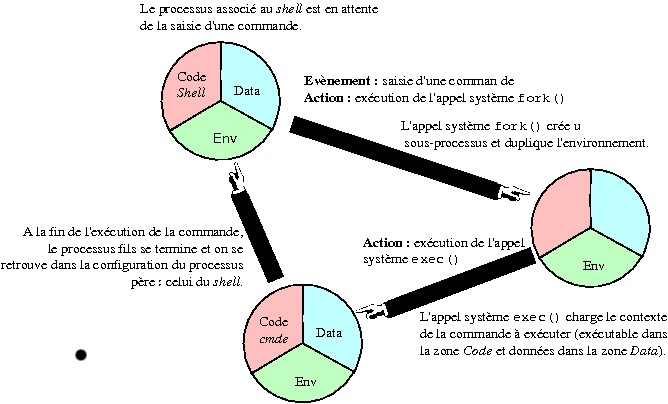
\includegraphics{./_Images/basic-notions/exec-cmd.jpg}
\caption{\label{fig-basnot-exec-cmd}Ex{\'e}cution d'une commande sous {\Unix}}
\end{figure}

L'appel syst{\`e}me "\texttt{fork()}" cr{\'e}e le processus et ne garde
que la zone m{\'e}moire "\texttt{ENV}". L'appel syst{\`e}me
"\texttt{exec()}" ex{\'e}cute la commande dans le processus cr{\'e}{\'e}.

\begin{remarque}
"\texttt{exec}" est aussi une commande du shell qui a la m{\^e}me fonctionnalit{\'e}.
\end{remarque}

La commande "\verb=% exec ls=" ex{\'e}cute "\texttt{ls}" dans le m{\^e}me processus
du shell (substitue le code du shell par le code de la commande "\texttt{ls}"
dans la zone m{\'e}moire "\texttt{CODE}" et s'arr{\^e}te d{\`e}s que son ex{\'e}cution est
termin{\'e}e. {\bf On est donc d{\'e}logg{\'e}}.

%%%%%%%%%%%%
\subsection{Les commandes de gestion des variables du shell}

\begin{definition}{Syntaxe}
\begin{tabular}{@{\hspace{1cm}}l}
	\texttt{set}\\[0.2cm]
	\texttt{variable=\textsl{valeur}}\\[0.2cm]
	\texttt{unset \textsl{variable}}\\[0.2cm]
	\texttt{export \textsl{variable}}\\[0.2cm]
	\texttt{printenv}\\[0.2cm]
	\texttt{env}\\
\end{tabular}
\end{definition}

\index{variable!gestion}
La commande \index{set@\texttt{set}}"\texttt{set}" sans argurments
affiche la liste des variables locales au shell

La commande \index{unset@\texttt{unset}}"\texttt{unset}" suivi d'un nom de variable permet
d'effacer celle-ci de la zone des variables locales du shell.

La commande \index{export@\texttt{export}}"\texttt{export}" suivie du nom d'une variable, permet de
placer une variable d{\'e}finie de la zone locale au shell vers la zone
d'environnement (exportation de la variable).

Les commandes \index{env@\texttt{env}}"\texttt{env}" et
\index{printenv@\texttt{printenv}}"\texttt{printenv}" listent les variables de la
zone d'environnement et les valeurs qui leur sont affect{\'e}es.

%%%%%%%%%%%
\subsection{Variables usuelles}

Le tableau \ref{tab-basnot-variables} donne la liste des
\index{variable!usuelle}variables les plus usuelles du shell {\Unix}.

\begin{longtable}{|l|p{8cm}|}
	\hline
	\multicolumn{2}{|r|}{Suite de la page pr{\'e}c{\'e}dente.} \\
	\hline
	\multicolumn{1}{|c|}{\textsl{Variable}}		&
	\multicolumn{1}{|c|}{\textsl{Signification}}	\\
	\hline
\endhead
	\hline
	\multicolumn{1}{|c|}{\textsl{Variable}}		&
	\multicolumn{1}{|c|}{\textsl{Signification}}	\\
	\hline
\endfirsthead
	\hline
\endfoot
	\hline
\endlastfoot
		\index{variable!PATH@\texttt{PATH}}\texttt{PATH}	&
		R{\'e}f{\'e}rence les chemins d'acc{\`e}s scrut{\'e}s lors de l'ex{\'e}cution d'une commande.\\
	\hline
		\index{variable!HOME@\texttt{HOME}}\texttt{HOME}	&
		R{\'e}f{\'e}rence le r{\'e}pertoire de \textsl{login}. C'est le r{\'e}pertoire par d{\'e}faut de la
		commande "\texttt{cd}".\\
	\hline
		\index{variable!PS1@\texttt{PS1}}\texttt{PS1}	&
		Invite du shell.\\
	\hline
		\index{variable!PS2@\texttt{PS2}}\texttt{PS2}	&
		Invite secondaire du shell. Lorsque vous demandez {\`a} ce qu'une commande se
		poursuive apr{\`e}s un retour chariot, c'est le contenu de cette de cette
		variable qui sera affich{\'e}.\\
	\hline
		\index{variable!LANG@\texttt{LANG}}\texttt{LANG}	&
		Langue utilis{\'e}e pour les messages.\\
	\hline
		\index{variable!HISTSIZE@\texttt{HISTSIZE}}\texttt{HISTSIZE}	&
		Nombre de commandes {\`a} m{\'e}moriser dans l'historique (Korn Shell uniquement).\\
	\hline
\caption{\label{tab-basnot-variables}Liste des variables les plus usuelles.}
\end{longtable}

%%%%%%%%%%%
\subsection{Visualisation d'une variable}

Pour rappeler le contenu d'une \index{variable!visualisation}variable
(locale ou d'environnement), il suffit de faire pr{\'e}c{\'e}der son nom
par le caract{\`e}re \index{\$@\texttt{\$}}"\texttt{\$}". Par cons{\'e}quent~:
\begin{itemize}
	\item pour r{\'e}f{\'e}rencer la variable, il suffit de pr{\'e}ciser son nom.
	\item pour r{\'e}f{\'e}rencer son contenu, il suffit de pr{\'e}ciser son nom pr{\'e}c{\'e}d{\'e} du
		  caract{\`e}re "\texttt{\$}".
\end{itemize}

\begin{example}
\begin{verbatim}
sh_ksh% my_var=schmoll
sh_ksh% echo $my_var
schmoll
\end{verbatim}
\end{example}

%%%%%%%%%%%%%%%%%%%%%%%%%%%%%%%%%%%%%%%%%%%%%%%%%%%%%%%%%%%%%%%%%%%%%
\section{\label{basicnot-exec}Ex{\'e}cution d'une commande}

La plupart des commandes sont des ex{\'e}cutables plac{\'e}s dans
\texttt{/bin}, \texttt{/sbin}, \texttt{/usr/bin}, \texttt{/usr/sbin},
etc. Ce sont des commandes {\Unix} ou
\index{commande!externe}\textbf{commandes externes au shell}. D'autres
commandes comme "\texttt{cd}", "\texttt{echo}",
"\texttt{pwd}" font partie intgrante de l'interpr{\'e}teur de commandes.
Ce sont des \index{commande!interne}\textbf{commandes internes au shell}.

Les commandes {\Unix} sont ex{\'e}cut{\'e}es dans un sous processus.
Comme les ex{\'e}cutables peuvent se trouver dans diff{\'e}rents
r{\'e}pertoires, le shell doit savoir o{\`u} les chercher. C'est la
variable "\index{variable!PATH@\texttt{PATH}}\texttt{PATH}" qui
d{\'e}finit la liste des r{\'e}pertoires {\`a} scruter et l'ordre dans
lequel le shell doit faire la recherche.

\begin{remarque}
Les commandes internes au shell ne sont pas ex{\'e}cut{\'e}es dans un processus fils.
\end{remarque}

%%%%%%%%%%%%%%%%%%%%%%%%%%%%%%%%%%%%%%%%%%%%%%%%%%%%%%%%%%%%%%%%%%%%%
\section{\label{redirect-io}Redirection des entr{\'e}es/sorties}

%%%%%%%%%%%
\subsection{Introduction}

Chaque processus sous {\Unix} poss{\'e}de trois canaux de communication~:
\begin{center}
\begin{tabular}{|l|c|c|c|}
	\hline
		\multicolumn{1}{|c|}{Canal de communication}	&
		Fichier											&
		Num{\'e}ro logique								&
		Analogie {\OpenVMS}								\\
	\hline \hline
		Entr{\'e}e standard								&
		\texttt{stdin}									&
		\texttt{0}										&
		\texttt{SYS\$INPUT}								\\
	\hline
		Sortie standard									&
		\texttt{stdout}									&
		\texttt{1}										&
		\texttt{SYS\$OUTPUT}							\\
	\hline
		Sortie d'erreurs standard						&
		\texttt{stderr}									&
		\texttt{2}										&
		\texttt{SYS\$ERROR}								\\
	\hline
\end{tabular}
\end{center}

La redirection de ces canaux est tr{\`e}s utilis{\'e}e sous {\Unix}. En
effet, beaucoup de commandes {\'e}crivent leur r{\'e}sultat par d{\'e}faut sur la
sortie standard (comme les filtres, par exemple). Le seul moyen de l'avoir
dans un fichier est de rediriger la sortie standard.
D'autres commandes lisent syst{\'e}matiquement sur leur entr{\'e}e standard
(comme les filtres). Si l'on veut qu'elles prennent un fichier comme
argument, il faudra rediriger l'entr{\'e}e standard.

Les syntaxes utilis{\'e}es pour les redirections sont explicit{\'e}es aux sections
\ref{basnot-stdin}, \ref{basnot-stdout} et \ref{basnot-stderr}.

%%%%%%%%%%%
\subsection{\label{basnot-stdin}Redirection de l'entr{\'e}e standard (\texttt{stdin})}

\begin{definition}{Syntaxe}
\begin{verbatim}
commande < nouvelle-entree-standard
\end{verbatim}
\end{definition}

Il est possible de rediriger l'entr{\'e}e de toute commande devant lire
des donn{\'e}es depuis \index{stdin@\texttt{stdin} (entr{\'e}e
standard)}l'entr{\'e}e standard, afin que la lecture se fasse sur un
fichier gr{\^a}ce au symbole \index{<@\verb=<=}"\verb=<=".

\begin{example}
\begin{verbatim}
% mail machin < fichier
\end{verbatim}
\end{example}

%%%%%%%%%%%%
\subsection{\label{basnot-stdout}Redirection de la sortie standard (\texttt{stdout})}

\begin{definition}{Syntaxe}
\begin{tabular}{l@{\hspace{1cm}}l}
	\verb=commande > nouvelle-sortie=	&	(Cr{\'e}ation/R{\'e}{\'e}criture)	\\
	\verb=commande >> nouvelle-sortie=	&	(Ajout)					\\
\end{tabular}
\end{definition}

Il est possible de rediriger la \index{stdout@\texttt{stdout} (sortie standard)}sortie
de toute commande devant {\'e}crire sur la sortie standard afin que l'{\'e}criture se fasse sur un fichier.
L'{\'e}criture peut se faire de deux fa\c{c}ons~:
\begin{itemize}
	\item	{\'e}criture dans un fichier et {\'e}crasement si le fichier existe d{\'e}j{\`a},
	\item	{\'e}criture {\`a} la suite d'un fichier d{\'e}j{\`a} existant.
\end{itemize}

Si une ligne de commande contient le symbole de redirection de la sortie
standard \index{>@\verb=>=}"\verb=>=" suivi d'un nom de fichier, celle-ci sera
redirig{\'e}e dans le fichier sp{\'e}cifi{\'e} au lieu du terminal. Deux cas peuvent
se pr{\'e}senter~:
\begin{itemize}
	\item	Si le fichier n'existe pas au moment o{\`u} la commande est ex{\'e}cut{\'e}e,
			il est cr{\'e}{\'e}.
	\item	Si le fichier existait, alors son contenu est {\'e}cras{\'e} par la sortie standard
			de la commande. Si on souhaite que celle-ci vienne s'ajouter {\`a} la suite,
			afin de pr{\'e}server son contenu initial, il suffit d'utiliser le double symbole
			"\verb=>>=". Dans le cas o{\`u} le fichier n'existait pas, il sera cr{\'e}{\'e}.
\end{itemize}

\begin{example}
\begin{verbatim}
% ls > fic
% date > who.log
% who >> who.log
\end{verbatim}
\end{example}

%%%%%%%%%%%%
\subsection{\label{basnot-stderr}Redirection de la sortie d'erreurs standard (\texttt{stderr})}

\begin{definition}{Syntaxe}
\begin{tabular}{l@{\hspace{1cm}}l}
	\verb=commande 2>fichier=	&	(Cr{\'e}ation/R{\'e}{\'e}criture)\\
	\verb=commande 2>>fichier=	&	(Ajout)\\
\end{tabular}
\end{definition}

La plupart des commandes {\Unix} produisent des messages de diagnostic
si un probl{\`e}me survient en cours d'ex{\'e}cution. La sortie des
messages d'erreur se fait sur la \index{stderr@\texttt{stderr} (sortie
d'erreurs standard)}sortie d'erreurs standard, qui, par d{\'e}faut, est
associ{\'e}e {\`a} l'{\'e}cran.

La sortie de messages d'erreur peut {\^e}tre redirig{\'e}e ind{\'e}pendamment de la
sortie standard. Ceci {\'e}vite d'avoir les messages d'ex{\'e}cution normale et
les messages de diagnostic entrelac{\'e}s dans un m{\^e}me fichier.

Pour rediriger la sortie d'erreurs standard dans un fichier, on utilise
les cha{\^\i}nes \index{>@\verb=>=}"\verb=2>=" et "\verb=2>>=" suivie du nom du fichier. Il ne doit
pas y avoir d'espace entre le "\texttt{2}" et le "\verb=>=". Comme pour la
redirection de la sortie standard, si le fichier n'existe pas, il est
cr{\'e}{\'e}, sinon il est {\'e}cras{\'e}. Si l'on veut que les messages de diagnostics
viennent s'ajouter en fin de fichier, il faut utiliser le double symbole
de redirection "\verb=2>>=".

\begin{example}
\begin{verbatim}
sh% cp fic1 fic2 2>fic
sh% cp fic1 fic2 2>>fic
\end{verbatim}
\end{example}

%%%%%%%%%%%
\subsection{Redirection d'une sortie standard vers une autre sortie standard}

Le principe reste identique. Il suffit de rediriger une sortie vers un
fichier (ou canal logique). Lorsque l'on veut r{\'e}f{\'e}rencer le canal
associ{\'e} {\`a} une sortie standard (idem pour l'entr{\'e}e et la sortie d'erreurs
standard) comme un fichier, il suffit de faire pr{\'e}c{\'e}d{\'e} son num{\'e}ro
logique par le caract{\`e}re <<\texttt{\&}".

Par exemple, si la \index{stderr@\texttt{stderr} (sortie d'erreurs
standard)}sortie d'erreurs standard doit {\^e}tre redirig{\'e}e vers la
\index{stdout@\texttt{stdout} (sortie standard)}sortie standard, il
suffira d'{\'e}crire~:
\begin{verbatim}
commande 2>&1
\end{verbatim}

Dans le cas o{\`u} la sortie standard et la sortie d'erreurs standard doivent {\^e}tre redirig{\'e}es
vers un m{\^e}me fichier, il faudra bien analyser le processus {\`a} mettre en jeu.

Dans le premier cas~:
\begin{center}
	\fbox{\texttt{commande 2>\&1 >fichier}}
\end{center}
le shell va ex{\'e}cuter les {\'e}tapes suivantes~:\\[0.5cm]
%	\epsfbox{_Images/basic-notions/stdout-stderr-1.eps}	\\
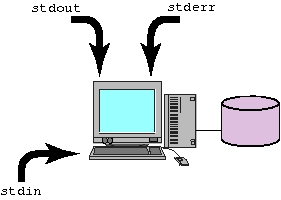
\includegraphics{./_Images/basic-notions/stdout-stderr-1.jpg}	\\
la sortie d'erreurs standard est redirig{\'e}e vers la valeur courante de la sortie
standard, {\bf donc l'{\'e}cran}.\\[0.5cm]
%\epsfbox{_Images/basic-notions/stdout-stderr-2.eps}	\\
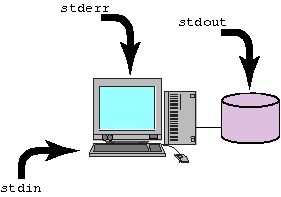
\includegraphics{./_Images/basic-notions/stdout-stderr-2.jpg} \\
la sortie standard vers un fichier. {\bf Donc seule la sortie standard a
{\'e}t{\'e} redirig{\'e}e vers un fichier}.

Dans le deuxi{\`e}me cas~:
\begin{center}
	\fbox{\texttt{commande >fichier 2>\&1}}
\end{center}
le shell va ex{\'e}cuter les {\'e}tapes suivantes~:\\[0.5cm]
%	\epsfbox{_Images/basic-notions/stdout-stderr-2.eps}	\\
	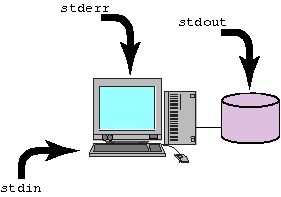
\includegraphics{./_Images/basic-notions/stdout-stderr-2.jpg}	\\
la sortie standard est redirig{\'e}e vers un fichier,\\[0.5cm]
%	\epsfbox{_Images/basic-notions/stdout-stderr-3.eps}	\\
	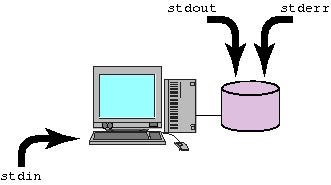
\includegraphics{./_Images/basic-notions/stdout-stderr-3.jpg}
la sortie d'erreurs standard est redirig{\'e}e vers la valeur courante sur laquelle
pointe la sortie standard, {\bf donc le fichier}. En cons{\'e}quence,
{\bf la sortie standard et la sortie d'erreurs standard ont bien {\'e}t{\'e} redirig{\'e}es vers un
m{\^e}me fichier}.

Le second mod{\`e}le est donc celui {\`a} retenir.

%%%%%%%%%%%%
\subsection{Redirection de la sortie standard d'une commande dans
		l'entr{\'e}e standard d'une autre}

\begin{definition}{Syntaxe}
\begin{tabular}{ccc}
	\textsl{Commande A}				&	\texttt{|}	&	\textsl{Commande B}	\\
	Doit {\'e}crire sur \texttt{stdout}	&			&	Doit lire sur \texttt{stdin}\\
\end{tabular}
\end{definition}

Le symbole \index{|@\texttt{|}}"\texttt{|}" appel{\'e} \index{pipe}"\textsl{pipe}", est
utilis{\'e} pour relier deux commandes entre elles. La
\index{stdout@\texttt{stdout} (sortie standard)}sortie standard de la
commande {\`a} gauche du symbole "\texttt{|}" est utilis{\'e}e comme
\index{stdin@\texttt{stdin} (entr{\'e}e standard)}entr{\'e}e standard de
la commande de droite. La figure \ref{fig-basnot-out2in} illustre le
principe utilis{\'e} pour ce type de redirection.

\begin{figure}[hbtp]
	\centering
%	\epsfbox{_Images/basic-notions/out2in.eps}	\\
	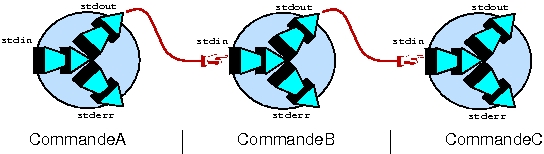
\includegraphics{./_Images/basic-notions/out2in.jpg}
	\caption{\label{fig-basnot-out2in}Enchainement de commandes, m{\'e}canisme du \textsl{pipe}.}
\end{figure}

C'est pourquoi~:
\begin{itemize}
	\item	toute commande situ{\'e}e {\`a} gauche du symbole "\texttt{|}" doit produire une
			sortie sur "\texttt{stdout}",
	\item	toute commande situ{\'e}e {\`a} droite du symbole "\texttt{|}" doit effectuer une
			lecture depuis "\texttt{stdin}",
	\item	toute commande entre les deux symboles "\texttt{|}" doit {\'e}crire sur
			"\texttt{stdout}" et lire sur "\texttt{stdin}". {\bf C'est donc un filtre}.
\end{itemize}

La redirection d'entr{\'e}e/sortie permet le passage d'informations entre un
processus et un fichier. Les \textsl{pipes} permettent le passage d'informations
entre processus. Ils constituent une solution pour utiliser la
sortie d'une commande en entr{\'e}e d'une autre commande sans passer par un
fichier interm{\'e}diaire.

{\Unix} repose sur le principe suivant. Chaque commande doit r{\'e}aliser
une seule chose. C'est la combinaison de ces commandes {\'e}l{\'e}mentaires,
gr{\^a}ce au m{\'e}canisme des \textsl{pipes} qui permet l'obtention de r{\'e}sultats
{\'e}labor{\'e}s.

%%%%%%%%%%%%%%%%%%%%%%%%%%%%%%%%%%%%%%%%%%%%%%%%%%%%%%%%%%%%%%%%%%%%%
\section{\label{basic-metacars}G{\'e}n{\'e}ration de noms de fichiers - Les m{\'e}tacaract{\`e}res}

%%%%%%%%%%%
\subsection{Introduction}

Les \index{m{\'e}tacaract{\`e}re}m{\'e}tacaract{\`e}res ne sont pas des
\index{wildcard}"\textsl{wildcards}". Un wildcard est
interpr{\'e}t{\'e} par une commande pour g{\'e}n{\'e}rer certains noms
de fichiers. Par contre les m{\'e}tacaract{\`e}res sont
interpr{\'e}t{\'e}s directement par le shell \textbf{avant
l'ex{\'e}cution de la commande}. Celle-ci re\c{c}oit des noms de
fichiers, comme si vous les aviez tap{\'e}s au clavier.

Les m{\'e}tacaract{\`e}res ne sont pas une aide {\`a} la frappe au clavier.
Les m{\'e}tacaract{\`e}res disponibles sont~:~\\
\begin{tabular}{lp{8cm}}
	\index{?@\texttt{?}}\texttt{?}		&
	Masque un caract{\`e}re, sauf le point en premi{\`e}re position.\\[0.5cm]
	\index{[]@\texttt{[]}}\texttt{[]}		&
	D{\'e}finit une classe de caract{\`e}res~:
	\begin{tabular}{lp{5cm}}
		\index{-@\texttt{-}}\texttt{-}	& pour d{\'e}finir une suite,\\
		\index{!@\texttt{!}}\texttt{!}	& pour exprimer une exclusion
	\end{tabular}
	Aucun s{\'e}parateur n'est utilis{\'e} pour exprimer une liste.\\[0.5cm]
	\index{*@\texttt{*}}\texttt{*}		&
	Masque toutes cha{\^\i}nes de caract{\`e}res, sauf le point en premi{\`e}re position.
\end{tabular}

\begin{remarque}
Les expressions utilisant les m{\'e}tacaract{\`e}res suivent les r{\`e}gles des expressions r{\'e}guli{\`e}res
{\Unix}.
\end{remarque}

Les m{\'e}tacaract{\`e}res ne masquent jamais les fichiers cach{\'e}s. Le point en d{\'e}but du nom d'un
fichier doit {\^e}tre tap{\'e} explicitement.

Le tableau \ref{tab-basenot-equiv-meta} donne les {\'e}quivalences entre {\Unix}
{\OpenVMS} et {\DOS} pour l'utilisation des m{\'e}tacaract{\`e}res sous {\Unix}.

\begin{table}[hbtp]
\centering
\begin{tabular}{|c|c|c|}
	\hline
		{\Unix}		&	{\OpenVMS}				&	{\DOS}		\\
	\hline \hline
		\texttt{*}	&	\texttt{*}				&	\texttt{*}				\\
	\hline
		\texttt{?}	&	\texttt{\%}				&	\texttt{?}				\\
	\hline
		\texttt{[]}	&	pas d'{\'e}quivalence	&	pas d'{\'e}quivalence	\\
	\hline
\end{tabular}
\caption{\label{tab-basenot-equiv-meta}\'{E}quivalence pour l'utilisation des m{\'e}tacaract{\`e}res
entre {\Unix}, {\OpenVMS} et {\DOS}.}
\end{table}

%%%%%%%%%%%
\subsection{Utilisation du m{\'e}tacaract{\`e}re "\texttt{?}"}

Le point d'interrogation \index{?@\texttt{?}}"\texttt{?}" masque un
et un seul caract{\`e}re sauf le point en premi{\`e}re position.

\begin{example}
\begin{tabular}{l@{\hspace{0.5cm}}p{8cm}}
	\texttt{echo ???}	&	Masque tous les noms de fichiers {\`a} trois caract{\`e}res.\\
	\texttt{ls A?C}	&	Masque tous les noms de fichiers {\`a} trois caract{\`e}res, dont
						le premier est "\texttt{A}" et le dernier est "\texttt{C}".\\
\end{tabular}
\end{example}

%%%%%%%%%%%
\subsection{Utilisation des m{\'e}tacaract{\`e}res "\texttt{[]}"}

Les crochets ouvrants et fermants
\index{[]@\texttt{[]}}\texttt{[]}"\texttt{[]}" d{\'e}finissent une
classe de caract{\`e}res, dont un et un seul sera masqu{\'e}.

\begin{example}
\begin{tabular}{l@{\hspace{0.5cm}}p{8cm}}
	\texttt{echo [abc]??}		&	Tous les fichiers dont le nom fait 3 caract{\`e}res et dont la
								premi{\`e}re lettre est soit "\texttt{a}", soit "\texttt{b}",
								soit "\texttt{c}".\\[0.5cm]
	\texttt{echo ?[a-zA-Z]}	&	Tous les fichiers dont le nom fait 2 caract{\`e}res et dont
								le dernier caract{\`e}re est une lettre (majuscule ou minuscule).
								\\[0.5cm]
	\texttt{echo [!a-zA-Z]??}	&	Tous les fichiers dont le nom fait 3 caract{\`e}res et dont le
								premier n'est pas une lettre.\\
\end{tabular}
\end{example}

%%%%%%%%%%%
\subsection{Utilisation du m{\'e}tacaract{\`e}re "\texttt{*}"}

L'{\'e}toile \index{*@\texttt{*}}"\texttt{*}" masque toute
cha{\^\i}ne de caract{\`e}res, m{\^e}me vide, sauf le point en
premi{\`e}re position.

\begin{example}
\begin{verbatim}
echo *
echo .*
echo *a*
\end{verbatim}
etc.
\end{example}

%%%%%%%%%%%%%%%%%%%%%%%%%%%%%%%%%%%%%%%%%%%%%%%%%%%%%%%%%%%%%%%%%%%%%
\section{\label{basic-quotes}Les quotes et les caract{\`e}res sp{\'e}ciaux}

\subsection{Introduction}

Nous avons vu dans les paragraphes pr{\'e}c{\'e}dents, les caract{\`e}res sp{\'e}ciaux suivants~:

\begin{longtable}{l@{\hspace{0.2cm}}p{8cm}}
	\texttt{\$}		&	utilis{\'e} pour la substitution d'une variable,						\\
	\texttt{? [] *}	&	utilis{\'e}s pour la g{\'e}n{\'e}ration des noms de fichiers par le Shell,		\\
	\verb=< > >>=	&	utilis{\'e}s pour la redirection des entr{\'e}es/sorties,					\\
	\spacekey		&	utilis{\'e} comme s{\'e}parateur par le Shell,								\\
	\texttt{|}		&	utilis{\'e} dans les \textsl{pipes}.										\\
\end{longtable}

Le contexte ne suffit pas toujours {\`a} d{\'e}terminer quel sens donner au
caract{\`e}re. C'est pourquoi il est n{\'e}cessaire d'avoir un moyen permettant
d'{\'e}chapper au sens sp{\'e}cial du caract{\`e}re et forcer celui-ci {\`a} {\^e}tre
consid{\'e}r{\'e} comme tel. \textbf{C'est le m{\'e}canisme de recours aux quotes}.

%%%%%%%%%%%%
\subsection{Les caract{\`e}res d'{\'e}chappements}

\begin{description}
	\item[\textbf{\index{\@$\mathtt{\backslash}$}back slash "$\mathtt{\backslash}$"}]\mbox{}\\
	Annule la signification particuli{\`e}re du caract{\`e}re imm{\'e}diatement apr{\`e}s.\\[0.5cm]
	\textsl{Exemple~:}\\
	\begin{tabular}{l@{\hspace{0.5cm}}p{6cm}}
		\verb=echo \$ABC=			&	renvoie la cha{\^\i}ne "\texttt{\$ABC}".\\
		\verb=echo abc \=\returnkey	&	annule l'interpr{\'e}tation du "\verb=<RETURN>=", il n'y a
										donc pas d'interpr{\'e}tation de la commande d'o{\`u} l'apparition d'un
										"\textsl{prompt secondaire}" pour continuer la commande.\\
	\end{tabular}

	\item[\index{'@\texttt{'}}\textbf{simple quote "\texttt{'}"}]\mbox{}\\
	Annule l'interpr{\'e}tation de tous les caract{\`e}res {\`a} l'int{\'e}rieur des quotes {\`a} l'exception de la
	simple quote elle-m{\^e}me.\\[0.5cm]
	\textsl{Exemple~:}\\
	\begin{tabular}{l@{\hspace{0.5cm}}p{6cm}}
		\verb=echo '$ABC > Bonjour'=	&	renvoie la cha{\^\i}ne "\verb=$ABC > Bonjour=" {\`a} l'{\'e}cran.\\
	\end{tabular}

	\item[\index{''@\texttt{''}}\textbf{doubles quotes "\texttt{"}"}]\mbox{}\\
		Annule l'interpr{\'e}tation de tous les caract{\`e}res entre les doubles quotes, {\`a} l'exception des
		caract{\`e}res \verb=\=, \texttt{"}, \texttt{\$} et \texttt{`} (back quote).\\[0.5cm]
	\textsl{Exemple~:}\\
	\begin{tabular}{l@{\hspace{0.5cm}}p{6cm}}
		\texttt{ABC=Salut}	&	\\
		\verb=echo "$ABC > Bonjour"=	&
			\raisebox{2ex}[0pt]{renvoie la cha{\^\i}ne "\texttt{Salut > Bonjour}" {\`a} l'{\'e}cran.}\\
	\end{tabular}

\end{description}

%%%%%%%%%%%%
\subsection{R{\'e}sum{\'e}}

\begin{longtable}{|c|p{2.5cm}|p{5cm}|p{3cm}|}
	\hline
	\multicolumn{4}{|r|}{Suite de la page pr{\'e}c{\'e}dente.} \\
	\hline
	\multicolumn{1}{|c|}{Symbole}	&
	\multicolumn{1}{|c|}{Type}		&
	\multicolumn{1}{|c|}{Action}	&
	\multicolumn{1}{|c|}{Exception}	\\
	\hline
\endhead
	\hline
	\multicolumn{1}{|c|}{Symbole}	&
	\multicolumn{1}{|c|}{Type}		&
	\multicolumn{1}{|c|}{Action}	&
	\multicolumn{1}{|c|}{Exception}	\\
	\hline
\endfirsthead
	\hline
	\multicolumn{4}{|r|}{Suite page suivante $\cdots$} \\
	\hline
\endfoot
	\hline
\endlastfoot
	\index{\$@\texttt{\$}}\texttt{\$}	&	Caract{\`e}re sp{\'e}cial	&
		Substitue la valeur d'une variable.		&
		\multicolumn{1}{|c|}{\textsl{N.A.}}		\\
	\hline

	\index{>@\verb=>=}\verb=>=, \verb=>>=				&
		Caract{\`e}re sp{\'e}cial						&
		Redirige la sortie standard vers un fichier.	&
		\multicolumn{1}{|c|}{\textsl{N.A.}}				\\
	\hline

	\index{<@\verb=<=}\verb=<=	&	Caract{\`e}re sp{\'e}cial		&
		Redirige l'entr{\'e}e standard {\`a} partir d'un fichier.	&
		\multicolumn{1}{|c|}{\textsl{N.A.}}							\\
	\hline

	\index{|@\texttt{|}}\texttt{|}	&	Caract{\`e}re sp{\'e}cial	&
		Combine plusieurs commandes dans un \textsl{pipe}.			&
		\multicolumn{1}{|c|}{\textsl{N.A.}}							\\
	\hline

	\spacekey	&	Caract{\`e}re sp{\'e}cial	&
		D{\'e}limiteur dans une commande.		&
		\multicolumn{1}{|c|}{\textsl{N.A.}}		\\
	\hline

	\index{?@\texttt{?}}\texttt{?}	&	M{\'e}ta\-caract{\`e}re				&
		Masque un caract{\`e}re, sauf le point en premi{\`e}re position.	&
		\multicolumn{1}{|c|}{\textsl{N.A.}}									\\
	\hline

	\index{[]@\texttt{[]}}\texttt{[]}	&	M{\'e}ta\-caract{\`e}re		&
		D{\'e}finit une classe de caract{\`e}res {\`a} masquer.			&
		\multicolumn{1}{|c|}{\textsl{N.A.}}								\\
	\hline

	\index{*@\texttt{*}}\texttt{*}		&	M{\'e}ta\-caract{\`e}re	&
		Masque toutes cha{\^\i}nes de caract{\`e}res, sauf
		le point en premi{\`e}re position.							&
		\multicolumn{1}{|c|}{\textsl{N.A.}}							\\
	\hline

	\index{\@$\mathtt{\backslash}$}\verb=\= (\textsl{back slash})	&
		Caract{\`e}re d'{\'e}chap\-pement						&
		Annule l'interpr{\'e}tation du caract{\`e}re suivant.	&
		\multicolumn{1}{|c|}{\textsl{Aucune.}} 			\\
	\hline

	\index{'@\texttt{'}}\texttt{'} (\textsl{simple quote})		&
		Caract{\`e}re d'{\'e}chap\-pement						&
		Annule l'interpr{\'e}tation de tous les caract{\`e}res
		entre les "\texttt{'}".								&
		\multicolumn{1}{|c|}{\textsl{Aucune.}} 					\\
	\hline

	\index{''@\texttt{''}}\texttt{"} (\textsl{double quotes})		&
		Caract{\`e}re d'{\'e}chap\-pement						&
		Annule l'interpr{\'e}tation de tous les caract{\`e}res
		entre les "\texttt{"}".								&
		\verb=\= (\textsl{back slash}),
		"\texttt{\$}" (symbole dollar),
		"\texttt{"}" (double quotes),
		"\texttt{`}" (back quote).						\\
\end{longtable}

